\documentclass[1p]{elsarticle_modified}
%\bibliographystyle{elsarticle-num}

%\usepackage[colorlinks]{hyperref}
%\usepackage{abbrmath_seonhwa} %\Abb, \Ascr, \Acal ,\Abf, \Afrak
\usepackage{amsfonts}
\usepackage{amssymb}
\usepackage{amsmath}
\usepackage{amsthm}
\usepackage{scalefnt}
\usepackage{amsbsy}
\usepackage{kotex}
\usepackage{caption}
\usepackage{subfig}
\usepackage{color}
\usepackage{graphicx}
\usepackage{xcolor} %% white, black, red, green, blue, cyan, magenta, yellow
\usepackage{float}
\usepackage{setspace}
\usepackage{hyperref}

\usepackage{tikz}
\usetikzlibrary{arrows}

\usepackage{multirow}
\usepackage{array} % fixed length table
\usepackage{hhline}

%%%%%%%%%%%%%%%%%%%%%
\makeatletter
\renewcommand*\env@matrix[1][\arraystretch]{%
	\edef\arraystretch{#1}%
	\hskip -\arraycolsep
	\let\@ifnextchar\new@ifnextchar
	\array{*\c@MaxMatrixCols c}}
\makeatother %https://tex.stackexchange.com/questions/14071/how-can-i-increase-the-line-spacing-in-a-matrix
%%%%%%%%%%%%%%%

\usepackage[normalem]{ulem}

\newcommand{\msout}[1]{\ifmmode\text{\sout{\ensuremath{#1}}}\else\sout{#1}\fi}
%SOURCE: \msout is \stkout macro in https://tex.stackexchange.com/questions/20609/strikeout-in-math-mode

\newcommand{\cancel}[1]{
	\ifmmode
	{\color{red}\msout{#1}}
	\else
	{\color{red}\sout{#1}}
	\fi
}

\newcommand{\add}[1]{
	{\color{blue}\uwave{#1}}
}

\newcommand{\replace}[2]{
	\ifmmode
	{\color{red}\msout{#1}}{\color{blue}\uwave{#2}}
	\else
	{\color{red}\sout{#1}}{\color{blue}\uwave{#2}}
	\fi
}

\newcommand{\Sol}{\mathcal{S}} %segment
\newcommand{\D}{D} %diagram
\newcommand{\A}{\mathcal{A}} %arc


%%%%%%%%%%%%%%%%%%%%%%%%%%%%%5 test

\def\sl{\operatorname{\textup{SL}}(2,\Cbb)}
\def\psl{\operatorname{\textup{PSL}}(2,\Cbb)}
\def\quan{\mkern 1mu \triangleright \mkern 1mu}

\theoremstyle{definition}
\newtheorem{thm}{Theorem}[section]
\newtheorem{prop}[thm]{Proposition}
\newtheorem{lem}[thm]{Lemma}
\newtheorem{ques}[thm]{Question}
\newtheorem{cor}[thm]{Corollary}
\newtheorem{defn}[thm]{Definition}
\newtheorem{exam}[thm]{Example}
\newtheorem{rmk}[thm]{Remark}
\newtheorem{alg}[thm]{Algorithm}

\newcommand{\I}{\sqrt{-1}}
\begin{document}

%\begin{frontmatter}
%
%\title{Boundary parabolic representations of knots up to 8 crossings}
%
%%% Group authors per affiliation:
%\author{Yunhi Cho} 
%\address{Department of Mathematics, University of Seoul, Seoul, Korea}
%\ead{yhcho@uos.ac.kr}
%
%
%\author{Seonhwa Kim} %\fnref{s_kim}}
%\address{Center for Geometry and Physics, Institute for Basic Science, Pohang, 37673, Korea}
%\ead{ryeona17@ibs.re.kr}
%
%\author{Hyuk Kim}
%\address{Department of Mathematical Sciences, Seoul National University, Seoul 08826, Korea}
%\ead{hyukkim@snu.ac.kr}
%
%\author{Seokbeom Yoon}
%\address{Department of Mathematical Sciences, Seoul National University, Seoul, 08826,  Korea}
%\ead{sbyoon15@snu.ac.kr}
%
%\begin{abstract}
%We find all boundary parabolic representation of knots up to 8 crossings.
%
%\end{abstract}
%\begin{keyword}
%    \MSC[2010] 57M25 
%\end{keyword}
%
%\end{frontmatter}

%\linenumbers
%\tableofcontents
%
\newcommand\colored[1]{\textcolor{white}{\rule[-0.35ex]{0.8em}{1.4ex}}\kern-0.8em\color{red} #1}%
%\newcommand\colored[1]{\textcolor{white}{ #1}\kern-2.17ex	\textcolor{white}{ #1}\kern-1.81ex	\textcolor{white}{ #1}\kern-2.15ex\color{red}#1	}

{\Large $\underline{12a_{1090}~(K12a_{1090})}$}

\setlength{\tabcolsep}{10pt}
\renewcommand{\arraystretch}{1.6}
\vspace{1cm}\begin{tabular}{m{100pt}>{\centering\arraybackslash}m{274pt}}
\multirow{5}{120pt}{
	\centering
	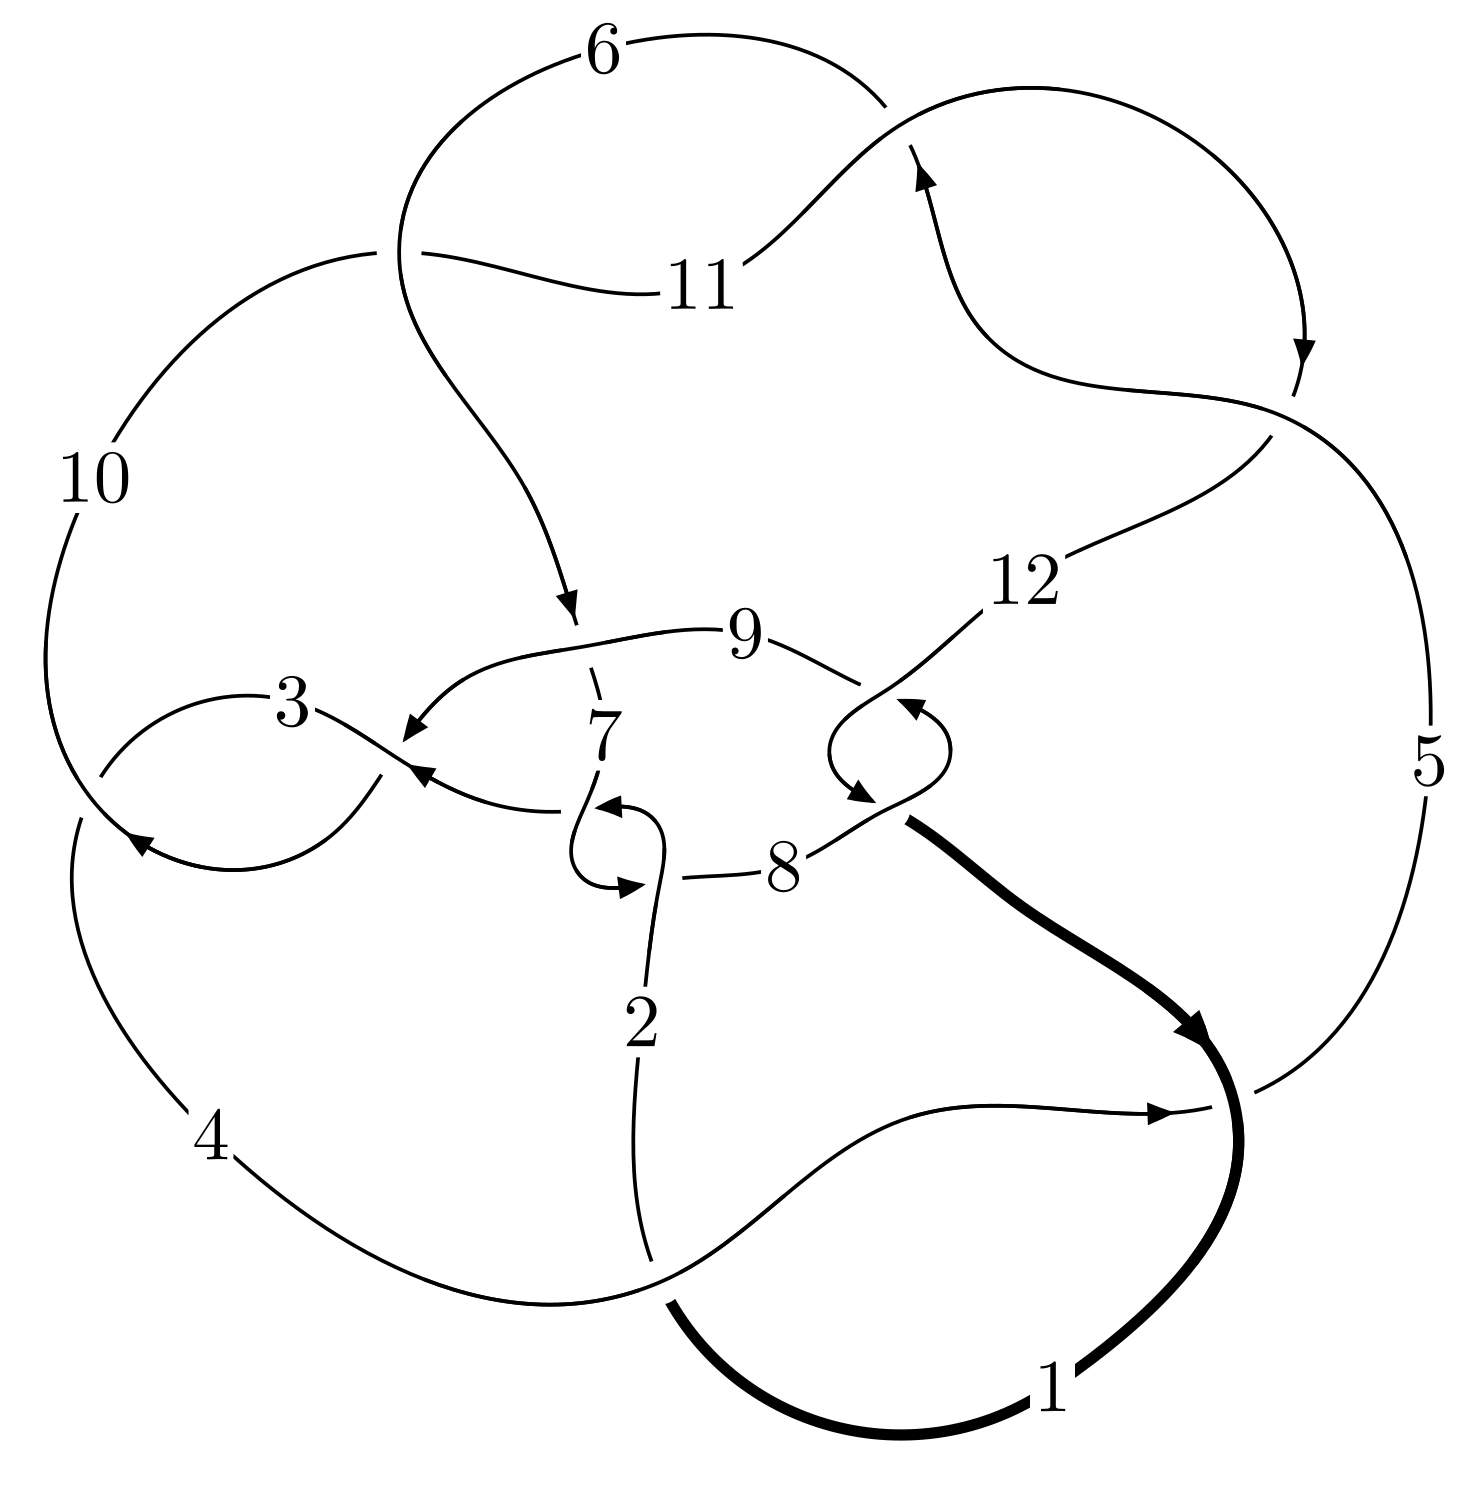
\includegraphics[width=112pt]{../../../GIT/diagram.site/Diagrams/png/1891_12a_1090.png}\\
\ \ \ A knot diagram\footnotemark}&
\allowdisplaybreaks
\textbf{Linearized knot diagam} \\
\cline{2-2}
 &
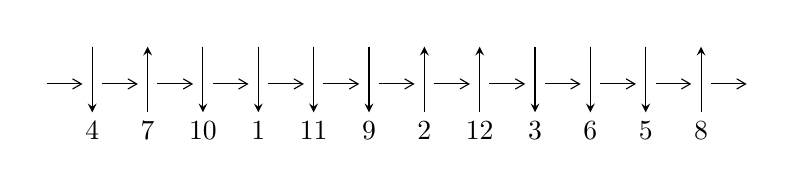
\begin{tikzpicture}[x=20pt, y=17pt]
	% nodes
	\node (C0) at (0, 0) {};
	\node (C1) at (1, 0) {};
	\node (C1U) at (1, +1) {};
	\node (C1D) at (1, -1) {4};

	\node (C2) at (2, 0) {};
	\node (C2U) at (2, +1) {};
	\node (C2D) at (2, -1) {7};

	\node (C3) at (3, 0) {};
	\node (C3U) at (3, +1) {};
	\node (C3D) at (3, -1) {10};

	\node (C4) at (4, 0) {};
	\node (C4U) at (4, +1) {};
	\node (C4D) at (4, -1) {1};

	\node (C5) at (5, 0) {};
	\node (C5U) at (5, +1) {};
	\node (C5D) at (5, -1) {11};

	\node (C6) at (6, 0) {};
	\node (C6U) at (6, +1) {};
	\node (C6D) at (6, -1) {9};

	\node (C7) at (7, 0) {};
	\node (C7U) at (7, +1) {};
	\node (C7D) at (7, -1) {2};

	\node (C8) at (8, 0) {};
	\node (C8U) at (8, +1) {};
	\node (C8D) at (8, -1) {12};

	\node (C9) at (9, 0) {};
	\node (C9U) at (9, +1) {};
	\node (C9D) at (9, -1) {3};

	\node (C10) at (10, 0) {};
	\node (C10U) at (10, +1) {};
	\node (C10D) at (10, -1) {6};

	\node (C11) at (11, 0) {};
	\node (C11U) at (11, +1) {};
	\node (C11D) at (11, -1) {5};

	\node (C12) at (12, 0) {};
	\node (C12U) at (12, +1) {};
	\node (C12D) at (12, -1) {8};
	\node (C13) at (13, 0) {};

	% arrows
	\draw[->,>={angle 60}]
	(C0) edge (C1) (C1) edge (C2) (C2) edge (C3) (C3) edge (C4) (C4) edge (C5) (C5) edge (C6) (C6) edge (C7) (C7) edge (C8) (C8) edge (C9) (C9) edge (C10) (C10) edge (C11) (C11) edge (C12) (C12) edge (C13) ;	\draw[->,>=stealth]
	(C1U) edge (C1D) (C2D) edge (C2U) (C3U) edge (C3D) (C4U) edge (C4D) (C5U) edge (C5D) (C6U) edge (C6D) (C7D) edge (C7U) (C8D) edge (C8U) (C9U) edge (C9D) (C10U) edge (C10D) (C11U) edge (C11D) (C12D) edge (C12U) ;
	\end{tikzpicture} \\
\hhline{~~} \\& 
\textbf{Solving Sequence} \\ \cline{2-2} 
 &
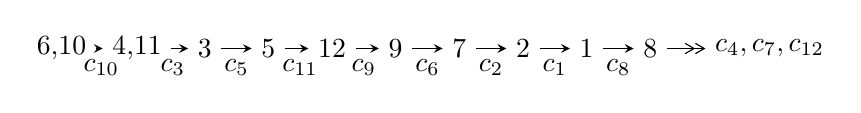
\begin{tikzpicture}[x=23pt, y=7pt]
	% node
	\node (A0) at (-1/8, 0) {6,10};
	\node (A1) at (17/16, 0) {4,11};
	\node (A2) at (17/8, 0) {3};
	\node (A3) at (25/8, 0) {5};
	\node (A4) at (33/8, 0) {12};
	\node (A5) at (41/8, 0) {9};
	\node (A6) at (49/8, 0) {7};
	\node (A7) at (57/8, 0) {2};
	\node (A8) at (65/8, 0) {1};
	\node (A9) at (73/8, 0) {8};
	\node (C1) at (1/2, -1) {$c_{10}$};
	\node (C2) at (13/8, -1) {$c_{3}$};
	\node (C3) at (21/8, -1) {$c_{5}$};
	\node (C4) at (29/8, -1) {$c_{11}$};
	\node (C5) at (37/8, -1) {$c_{9}$};
	\node (C6) at (45/8, -1) {$c_{6}$};
	\node (C7) at (53/8, -1) {$c_{2}$};
	\node (C8) at (61/8, -1) {$c_{1}$};
	\node (C9) at (69/8, -1) {$c_{8}$};
	\node (A10) at (11, 0) {$c_{4},c_{7},c_{12}$};

	% edge
	\draw[->,>=stealth]	
	(A0) edge (A1) (A1) edge (A2) (A2) edge (A3) (A3) edge (A4) (A4) edge (A5) (A5) edge (A6) (A6) edge (A7) (A7) edge (A8) (A8) edge (A9) ;
	\draw[->>,>={angle 60}]	
	(A9) edge (A10);
\end{tikzpicture} \\ 

\end{tabular} \\

\footnotetext{
The image of knot diagram is generated by the software ``\textbf{Draw programme}" developed by Andrew Bartholomew(\url{http://www.layer8.co.uk/maths/draw/index.htm\#Running-draw}), where we modified some parts for our purpose(\url{https://github.com/CATsTAILs/LinksPainter}).
}\phantom \\ \newline 
\centering \textbf{Ideals for irreducible components\footnotemark of $X_{\text{par}}$} 
 
\begin{align*}
I^u_{1}&=\langle 
1.10479\times10^{362} u^{116}+1.89977\times10^{362} u^{115}+\cdots+7.75796\times10^{363} b+1.93597\times10^{364},\\
\phantom{I^u_{1}}&\phantom{= \langle  }1.94516\times10^{364} u^{116}+1.50624\times10^{364} u^{115}+\cdots+7.29248\times10^{365} a+2.94268\times10^{365},\\
\phantom{I^u_{1}}&\phantom{= \langle  }u^{117}+u^{116}+\cdots+124 u+47\rangle \\
I^u_{2}&=\langle 
20149292 u^{29}-20623955 u^{28}+\cdots+99034091 b+23108758,\\
\phantom{I^u_{2}}&\phantom{= \langle  }-366097415 u^{29}+204883942 u^{28}+\cdots+792272728 a-2378612097,\;u^{30}+20 u^{28}+\cdots+2 u+1\rangle \\
\\
\end{align*}
\raggedright * 2 irreducible components of $\dim_{\mathbb{C}}=0$, with total 147 representations.\\
\footnotetext{All coefficients of polynomials are rational numbers. But the coefficients are sometimes approximated in decimal forms when there is not enough margin.}
\newpage
\renewcommand{\arraystretch}{1}
\centering \section*{I. $I^u_{1}= \langle 1.10\times10^{362} u^{116}+1.90\times10^{362} u^{115}+\cdots+7.76\times10^{363} b+1.94\times10^{364},\;1.95\times10^{364} u^{116}+1.51\times10^{364} u^{115}+\cdots+7.29\times10^{365} a+2.94\times10^{365},\;u^{117}+u^{116}+\cdots+124 u+47 \rangle$}
\flushleft \textbf{(i) Arc colorings}\\
\begin{tabular}{m{7pt} m{180pt} m{7pt} m{180pt} }
\flushright $a_{6}=$&$\begin{pmatrix}0\\u\end{pmatrix}$ \\
\flushright $a_{10}=$&$\begin{pmatrix}1\\0\end{pmatrix}$ \\
\flushright $a_{4}=$&$\begin{pmatrix}-0.0266735 u^{116}-0.0206547 u^{115}+\cdots-19.9608 u-0.403523\\-0.0142407 u^{116}-0.0244880 u^{115}+\cdots+0.591814 u-2.49546\end{pmatrix}$ \\
\flushright $a_{11}=$&$\begin{pmatrix}1\\u^2\end{pmatrix}$ \\
\flushright $a_{3}=$&$\begin{pmatrix}-0.0409142 u^{116}-0.0451426 u^{115}+\cdots-19.3690 u-2.89898\\-0.0142407 u^{116}-0.0244880 u^{115}+\cdots+0.591814 u-2.49546\end{pmatrix}$ \\
\flushright $a_{5}=$&$\begin{pmatrix}u\\u^3+u\end{pmatrix}$ \\
\flushright $a_{12}=$&$\begin{pmatrix}u^2+1\\u^4+2 u^2\end{pmatrix}$ \\
\flushright $a_{9}=$&$\begin{pmatrix}-0.00104818 u^{116}+0.0000285478 u^{115}+\cdots+23.6582 u-0.194678\\0.000577895 u^{116}-0.00548604 u^{115}+\cdots+3.54854 u-0.813912\end{pmatrix}$ \\
\flushright $a_{7}=$&$\begin{pmatrix}0.0378466 u^{116}+0.0626004 u^{115}+\cdots+26.8224 u+9.09236\\0.0394917 u^{116}+0.0258151 u^{115}+\cdots+4.33627 u+3.49687\end{pmatrix}$ \\
\flushright $a_{2}=$&$\begin{pmatrix}-0.0510015 u^{116}-0.0497058 u^{115}+\cdots-13.6495 u-3.84875\\-0.0278995 u^{116}-0.0302454 u^{115}+\cdots-5.89036 u-2.37136\end{pmatrix}$ \\
\flushright $a_{1}=$&$\begin{pmatrix}-0.0408163 u^{116}-0.0556002 u^{115}+\cdots-1.82172 u+0.570663\\-0.0448536 u^{116}-0.0160504 u^{115}+\cdots-4.25598 u-2.61750\end{pmatrix}$ \\
\flushright $a_{8}=$&$\begin{pmatrix}-0.00647050 u^{116}-0.00436844 u^{115}+\cdots+19.2576 u+0.614457\\0.000350157 u^{116}-0.00369785 u^{115}+\cdots+3.03710 u-1.22651\end{pmatrix}$\\&\end{tabular}
\flushleft \textbf{(ii) Obstruction class $= -1$}\\~\\
\flushleft \textbf{(iii) Cusp Shapes $= 0.126931 u^{116}+0.0615865 u^{115}+\cdots+15.3051 u+14.4162$}\\~\\
\newpage\renewcommand{\arraystretch}{1}
\flushleft \textbf{(iv) u-Polynomials at the component}\newline \\
\begin{tabular}{m{50pt}|m{274pt}}
Crossings & \hspace{64pt}u-Polynomials at each crossing \\
\hline $$\begin{aligned}c_{1},c_{4}\end{aligned}$$&$\begin{aligned}
&u^{117}-5 u^{116}+\cdots-1550 u+337
\end{aligned}$\\
\hline $$\begin{aligned}c_{2},c_{7}\end{aligned}$$&$\begin{aligned}
&u^{117}+u^{116}+\cdots-522928 u+122248
\end{aligned}$\\
\hline $$\begin{aligned}c_{3},c_{9}\end{aligned}$$&$\begin{aligned}
&u^{117}+u^{116}+\cdots+8557 u+3421
\end{aligned}$\\
\hline $$\begin{aligned}c_{5},c_{10},c_{11}\end{aligned}$$&$\begin{aligned}
&u^{117}+u^{116}+\cdots+124 u+47
\end{aligned}$\\
\hline $$\begin{aligned}c_{6}\end{aligned}$$&$\begin{aligned}
&u^{117}-3 u^{116}+\cdots+5055780 u-844876
\end{aligned}$\\
\hline $$\begin{aligned}c_{8},c_{12}\end{aligned}$$&$\begin{aligned}
&u^{117}-3 u^{116}+\cdots+34 u+31
\end{aligned}$\\
\hline
\end{tabular}\\~\\
\newpage\renewcommand{\arraystretch}{1}
\flushleft \textbf{(v) Riley Polynomials at the component}\newline \\
\begin{tabular}{m{50pt}|m{274pt}}
Crossings & \hspace{64pt}Riley Polynomials at each crossing \\
\hline $$\begin{aligned}c_{1},c_{4}\end{aligned}$$&$\begin{aligned}
&y^{117}+73 y^{116}+\cdots-8150992 y-113569
\end{aligned}$\\
\hline $$\begin{aligned}c_{2},c_{7}\end{aligned}$$&$\begin{aligned}
&y^{117}+93 y^{116}+\cdots-163687062112 y-14944573504
\end{aligned}$\\
\hline $$\begin{aligned}c_{3},c_{9}\end{aligned}$$&$\begin{aligned}
&y^{117}-65 y^{116}+\cdots+196939293 y-11703241
\end{aligned}$\\
\hline $$\begin{aligned}c_{5},c_{10},c_{11}\end{aligned}$$&$\begin{aligned}
&y^{117}+123 y^{116}+\cdots-54748 y-2209
\end{aligned}$\\
\hline $$\begin{aligned}c_{6}\end{aligned}$$&$\begin{aligned}
&y^{117}-27 y^{116}+\cdots-13642460366432 y-713815455376
\end{aligned}$\\
\hline $$\begin{aligned}c_{8},c_{12}\end{aligned}$$&$\begin{aligned}
&y^{117}+61 y^{116}+\cdots-60038 y-961
\end{aligned}$\\
\hline
\end{tabular}\\~\\
\newpage\flushleft \textbf{(vi) Complex Volumes and Cusp Shapes}
$$\begin{array}{c|c|c}  
\text{Solutions to }I^u_{1}& \I (\text{vol} + \sqrt{-1}CS) & \text{Cusp shape}\\
 \hline 
\begin{aligned}
u &= -0.450430 + 0.874019 I \\
a &= -0.155942 - 1.219730 I \\
b &= -0.988758 + 0.419017 I\end{aligned}
 & \phantom{-}1.31804 + 2.76130 I & \phantom{-0.000000 } 0 \\ \hline\begin{aligned}
u &= -0.450430 - 0.874019 I \\
a &= -0.155942 + 1.219730 I \\
b &= -0.988758 - 0.419017 I\end{aligned}
 & \phantom{-}1.31804 - 2.76130 I & \phantom{-0.000000 } 0 \\ \hline\begin{aligned}
u &= \phantom{-}0.375495 + 0.837694 I \\
a &= -0.724013 - 1.058100 I \\
b &= \phantom{-}1.164760 - 0.072289 I\end{aligned}
 & -2.40578 - 0.38438 I & \phantom{-0.000000 } 0 \\ \hline\begin{aligned}
u &= \phantom{-}0.375495 - 0.837694 I \\
a &= -0.724013 + 1.058100 I \\
b &= \phantom{-}1.164760 + 0.072289 I\end{aligned}
 & -2.40578 + 0.38438 I & \phantom{-0.000000 } 0 \\ \hline\begin{aligned}
u &= -0.709889 + 0.552874 I \\
a &= \phantom{-}0.198170 - 0.374731 I \\
b &= \phantom{-}0.366559 + 0.453634 I\end{aligned}
 & \phantom{-}0.98855 + 2.99976 I & \phantom{-0.000000 } 0 \\ \hline\begin{aligned}
u &= -0.709889 - 0.552874 I \\
a &= \phantom{-}0.198170 + 0.374731 I \\
b &= \phantom{-}0.366559 - 0.453634 I\end{aligned}
 & \phantom{-}0.98855 - 2.99976 I & \phantom{-0.000000 } 0 \\ \hline\begin{aligned}
u &= -0.980561 + 0.521676 I \\
a &= -0.304385 - 1.010160 I \\
b &= -1.32872 + 0.50810 I\end{aligned}
 & -6.2327 + 13.1746 I & \phantom{-0.000000 } 0 \\ \hline\begin{aligned}
u &= -0.980561 - 0.521676 I \\
a &= -0.304385 + 1.010160 I \\
b &= -1.32872 - 0.50810 I\end{aligned}
 & -6.2327 - 13.1746 I & \phantom{-0.000000 } 0 \\ \hline\begin{aligned}
u &= -0.581326 + 0.958709 I \\
a &= -0.160347 - 1.077050 I \\
b &= -0.997335 + 0.399940 I\end{aligned}
 & \phantom{-}1.30976 + 2.75887 I & \phantom{-0.000000 } 0 \\ \hline\begin{aligned}
u &= -0.581326 - 0.958709 I \\
a &= -0.160347 + 1.077050 I \\
b &= -0.997335 - 0.399940 I\end{aligned}
 & \phantom{-}1.30976 - 2.75887 I & \phantom{-0.000000 } 0\\
 \hline 
 \end{array}$$\newpage$$\begin{array}{c|c|c}  
\text{Solutions to }I^u_{1}& \I (\text{vol} + \sqrt{-1}CS) & \text{Cusp shape}\\
 \hline 
\begin{aligned}
u &= -0.727403 + 0.481710 I \\
a &= \phantom{-}0.84632 + 1.34115 I \\
b &= \phantom{-}1.254570 - 0.443656 I\end{aligned}
 & -9.34800 + 6.57460 I & \phantom{-0.000000 } 0 \\ \hline\begin{aligned}
u &= -0.727403 - 0.481710 I \\
a &= \phantom{-}0.84632 - 1.34115 I \\
b &= \phantom{-}1.254570 + 0.443656 I\end{aligned}
 & -9.34800 - 6.57460 I & \phantom{-0.000000 } 0 \\ \hline\begin{aligned}
u &= \phantom{-}0.842085 + 0.187380 I \\
a &= -0.425383 + 0.368443 I \\
b &= -1.228440 + 0.302698 I\end{aligned}
 & -3.96197 + 3.71063 I & \phantom{-0.000000 } 0 \\ \hline\begin{aligned}
u &= \phantom{-}0.842085 - 0.187380 I \\
a &= -0.425383 - 0.368443 I \\
b &= -1.228440 - 0.302698 I\end{aligned}
 & -3.96197 - 3.71063 I & \phantom{-0.000000 } 0 \\ \hline\begin{aligned}
u &= -0.522458 + 0.678849 I \\
a &= -0.293846 - 0.577453 I \\
b &= -1.122850 - 0.348363 I\end{aligned}
 & -8.82823 - 2.11501 I & \phantom{-0.000000 } 0 \\ \hline\begin{aligned}
u &= -0.522458 - 0.678849 I \\
a &= -0.293846 + 0.577453 I \\
b &= -1.122850 + 0.348363 I\end{aligned}
 & -8.82823 + 2.11501 I & \phantom{-0.000000 } 0 \\ \hline\begin{aligned}
u &= \phantom{-}0.448800 + 0.716787 I \\
a &= \phantom{-}1.36941 - 1.49722 I \\
b &= -0.449149 + 0.727366 I\end{aligned}
 & -0.91557 + 3.36877 I & \phantom{-0.000000 } 0 \\ \hline\begin{aligned}
u &= \phantom{-}0.448800 - 0.716787 I \\
a &= \phantom{-}1.36941 + 1.49722 I \\
b &= -0.449149 - 0.727366 I\end{aligned}
 & -0.91557 - 3.36877 I & \phantom{-0.000000 } 0 \\ \hline\begin{aligned}
u &= \phantom{-}0.747868 + 0.368257 I \\
a &= \phantom{-}0.076550 - 0.857149 I \\
b &= \phantom{-}0.007519 + 1.070980 I\end{aligned}
 & -2.03502 - 7.66434 I & \phantom{-0.000000 } 0 \\ \hline\begin{aligned}
u &= \phantom{-}0.747868 - 0.368257 I \\
a &= \phantom{-}0.076550 + 0.857149 I \\
b &= \phantom{-}0.007519 - 1.070980 I\end{aligned}
 & -2.03502 + 7.66434 I & \phantom{-0.000000 } 0\\
 \hline 
 \end{array}$$\newpage$$\begin{array}{c|c|c}  
\text{Solutions to }I^u_{1}& \I (\text{vol} + \sqrt{-1}CS) & \text{Cusp shape}\\
 \hline 
\begin{aligned}
u &= -0.819476 + 0.021910 I \\
a &= \phantom{-}0.175354 + 0.611821 I \\
b &= \phantom{-}1.41065 - 0.44823 I\end{aligned}
 & -6.62732 - 2.00391 I & \phantom{-0.000000 } 0 \\ \hline\begin{aligned}
u &= -0.819476 - 0.021910 I \\
a &= \phantom{-}0.175354 - 0.611821 I \\
b &= \phantom{-}1.41065 + 0.44823 I\end{aligned}
 & -6.62732 + 2.00391 I & \phantom{-0.000000 } 0 \\ \hline\begin{aligned}
u &= \phantom{-}1.149070 + 0.322405 I \\
a &= \phantom{-}0.624379 - 0.506587 I \\
b &= \phantom{-}0.964612 + 0.314051 I\end{aligned}
 & -0.55784 - 6.19834 I & \phantom{-0.000000 } 0 \\ \hline\begin{aligned}
u &= \phantom{-}1.149070 - 0.322405 I \\
a &= \phantom{-}0.624379 + 0.506587 I \\
b &= \phantom{-}0.964612 - 0.314051 I\end{aligned}
 & -0.55784 + 6.19834 I & \phantom{-0.000000 } 0 \\ \hline\begin{aligned}
u &= \phantom{-}0.301498 + 1.162040 I \\
a &= -0.26659 - 1.45212 I \\
b &= \phantom{-}0.974297 + 0.217920 I\end{aligned}
 & -0.995060 - 0.963784 I & \phantom{-0.000000 } 0 \\ \hline\begin{aligned}
u &= \phantom{-}0.301498 - 1.162040 I \\
a &= -0.26659 + 1.45212 I \\
b &= \phantom{-}0.974297 - 0.217920 I\end{aligned}
 & -0.995060 + 0.963784 I & \phantom{-0.000000 } 0 \\ \hline\begin{aligned}
u &= -0.273778 + 1.174630 I \\
a &= \phantom{-}1.114810 - 0.139072 I \\
b &= -1.55406 - 0.07468 I\end{aligned}
 & -3.14135 + 6.02194 I & \phantom{-0.000000 } 0 \\ \hline\begin{aligned}
u &= -0.273778 - 1.174630 I \\
a &= \phantom{-}1.114810 + 0.139072 I \\
b &= -1.55406 + 0.07468 I\end{aligned}
 & -3.14135 - 6.02194 I & \phantom{-0.000000 } 0 \\ \hline\begin{aligned}
u &= \phantom{-}0.600730 + 0.462863 I \\
a &= -0.568147 + 0.467016 I \\
b &= -0.003909 - 0.811777 I\end{aligned}
 & -5.54773 - 2.01439 I & \phantom{-0.000000 } 0 \\ \hline\begin{aligned}
u &= \phantom{-}0.600730 - 0.462863 I \\
a &= -0.568147 - 0.467016 I \\
b &= -0.003909 + 0.811777 I\end{aligned}
 & -5.54773 + 2.01439 I & \phantom{-0.000000 } 0\\
 \hline 
 \end{array}$$\newpage$$\begin{array}{c|c|c}  
\text{Solutions to }I^u_{1}& \I (\text{vol} + \sqrt{-1}CS) & \text{Cusp shape}\\
 \hline 
\begin{aligned}
u &= \phantom{-}0.589429 + 0.475259 I \\
a &= \phantom{-}0.487315 - 1.272170 I \\
b &= \phantom{-}1.34874 + 0.54161 I\end{aligned}
 & -2.94157 - 7.60929 I & \phantom{-0.000000 } 0 \\ \hline\begin{aligned}
u &= \phantom{-}0.589429 - 0.475259 I \\
a &= \phantom{-}0.487315 + 1.272170 I \\
b &= \phantom{-}1.34874 - 0.54161 I\end{aligned}
 & -2.94157 + 7.60929 I & \phantom{-0.000000 } 0 \\ \hline\begin{aligned}
u &= \phantom{-}0.733472 + 0.162116 I \\
a &= -1.090300 - 0.048396 I \\
b &= -1.141370 - 0.125034 I\end{aligned}
 & -4.04433 - 2.86679 I & \phantom{-0.000000 } 0 \\ \hline\begin{aligned}
u &= \phantom{-}0.733472 - 0.162116 I \\
a &= -1.090300 + 0.048396 I \\
b &= -1.141370 + 0.125034 I\end{aligned}
 & -4.04433 + 2.86679 I & \phantom{-0.000000 } 0 \\ \hline\begin{aligned}
u &= \phantom{-}0.265307 + 0.697351 I \\
a &= \phantom{-}0.095698 - 0.802970 I \\
b &= -0.453016 + 0.737857 I\end{aligned}
 & \phantom{-}2.93848 + 1.49224 I & \phantom{-0.000000 } 0 \\ \hline\begin{aligned}
u &= \phantom{-}0.265307 - 0.697351 I \\
a &= \phantom{-}0.095698 + 0.802970 I \\
b &= -0.453016 - 0.737857 I\end{aligned}
 & \phantom{-}2.93848 - 1.49224 I & \phantom{-0.000000 } 0 \\ \hline\begin{aligned}
u &= -0.419354 + 1.202530 I \\
a &= \phantom{-}0.63820 - 1.90195 I \\
b &= -1.208690 + 0.724572 I\end{aligned}
 & -2.84569 + 2.44067 I & \phantom{-0.000000 } 0 \\ \hline\begin{aligned}
u &= -0.419354 - 1.202530 I \\
a &= \phantom{-}0.63820 + 1.90195 I \\
b &= -1.208690 - 0.724572 I\end{aligned}
 & -2.84569 - 2.44067 I & \phantom{-0.000000 } 0 \\ \hline\begin{aligned}
u &= \phantom{-}0.708999 + 0.154308 I \\
a &= -0.801573 + 0.266034 I \\
b &= -1.314790 - 0.330863 I\end{aligned}
 & -4.59994 - 3.42538 I & \phantom{-0.000000 } 0 \\ \hline\begin{aligned}
u &= \phantom{-}0.708999 - 0.154308 I \\
a &= -0.801573 - 0.266034 I \\
b &= -1.314790 + 0.330863 I\end{aligned}
 & -4.59994 + 3.42538 I & \phantom{-0.000000 } 0\\
 \hline 
 \end{array}$$\newpage$$\begin{array}{c|c|c}  
\text{Solutions to }I^u_{1}& \I (\text{vol} + \sqrt{-1}CS) & \text{Cusp shape}\\
 \hline 
\begin{aligned}
u &= -0.077026 + 1.275020 I \\
a &= -0.38863 - 2.02126 I \\
b &= \phantom{-}0.17592 + 1.53970 I\end{aligned}
 & \phantom{-}4.66408 + 0.01829 I & \phantom{-0.000000 } 0 \\ \hline\begin{aligned}
u &= -0.077026 - 1.275020 I \\
a &= -0.38863 + 2.02126 I \\
b &= \phantom{-}0.17592 - 1.53970 I\end{aligned}
 & \phantom{-}4.66408 - 0.01829 I & \phantom{-0.000000 } 0 \\ \hline\begin{aligned}
u &= -0.043378 + 1.282440 I \\
a &= \phantom{-}0.081358 - 1.174000 I \\
b &= -1.165260 + 0.435563 I\end{aligned}
 & \phantom{-}1.86498 + 2.15332 I & \phantom{-0.000000 } 0 \\ \hline\begin{aligned}
u &= -0.043378 - 1.282440 I \\
a &= \phantom{-}0.081358 + 1.174000 I \\
b &= -1.165260 - 0.435563 I\end{aligned}
 & \phantom{-}1.86498 - 2.15332 I & \phantom{-0.000000 } 0 \\ \hline\begin{aligned}
u &= \phantom{-}0.099081 + 1.287910 I \\
a &= -0.239261 - 1.096180 I \\
b &= -0.137029 + 0.846959 I\end{aligned}
 & \phantom{-}3.68040 + 1.59802 I & \phantom{-0.000000 } 0 \\ \hline\begin{aligned}
u &= \phantom{-}0.099081 - 1.287910 I \\
a &= -0.239261 + 1.096180 I \\
b &= -0.137029 - 0.846959 I\end{aligned}
 & \phantom{-}3.68040 - 1.59802 I & \phantom{-0.000000 } 0 \\ \hline\begin{aligned}
u &= -1.038490 + 0.800183 I \\
a &= -0.192780 + 0.089886 I \\
b &= \phantom{-}1.244190 + 0.324174 I\end{aligned}
 & -5.58201 - 6.62080 I & \phantom{-0.000000 } 0 \\ \hline\begin{aligned}
u &= -1.038490 - 0.800183 I \\
a &= -0.192780 - 0.089886 I \\
b &= \phantom{-}1.244190 - 0.324174 I\end{aligned}
 & -5.58201 + 6.62080 I & \phantom{-0.000000 } 0 \\ \hline\begin{aligned}
u &= -0.202146 + 1.297420 I \\
a &= -0.862714 - 0.338807 I \\
b &= \phantom{-}1.36307 + 0.39085 I\end{aligned}
 & -3.82100 - 0.00691 I & \phantom{-0.000000 } 0 \\ \hline\begin{aligned}
u &= -0.202146 - 1.297420 I \\
a &= -0.862714 + 0.338807 I \\
b &= \phantom{-}1.36307 - 0.39085 I\end{aligned}
 & -3.82100 + 0.00691 I & \phantom{-0.000000 } 0\\
 \hline 
 \end{array}$$\newpage$$\begin{array}{c|c|c}  
\text{Solutions to }I^u_{1}& \I (\text{vol} + \sqrt{-1}CS) & \text{Cusp shape}\\
 \hline 
\begin{aligned}
u &= \phantom{-}0.130018 + 1.308590 I \\
a &= -0.16741 - 1.68093 I \\
b &= \phantom{-}1.32311 + 0.49998 I\end{aligned}
 & -0.68976 - 6.56572 I & \phantom{-0.000000 } 0 \\ \hline\begin{aligned}
u &= \phantom{-}0.130018 - 1.308590 I \\
a &= -0.16741 + 1.68093 I \\
b &= \phantom{-}1.32311 - 0.49998 I\end{aligned}
 & -0.68976 + 6.56572 I & \phantom{-0.000000 } 0 \\ \hline\begin{aligned}
u &= -0.073373 + 1.335250 I \\
a &= -0.95421 + 2.09276 I \\
b &= \phantom{-}1.09403 - 0.94824 I\end{aligned}
 & -4.70547 + 3.68035 I & \phantom{-0.000000 } 0 \\ \hline\begin{aligned}
u &= -0.073373 - 1.335250 I \\
a &= -0.95421 - 2.09276 I \\
b &= \phantom{-}1.09403 + 0.94824 I\end{aligned}
 & -4.70547 - 3.68035 I & \phantom{-0.000000 } 0 \\ \hline\begin{aligned}
u &= \phantom{-}0.075591 + 1.344550 I \\
a &= \phantom{-}0.56822 + 1.44412 I \\
b &= \phantom{-}0.982176 - 0.233908 I\end{aligned}
 & \phantom{-}3.39050 - 5.09084 I & \phantom{-0.000000 } 0 \\ \hline\begin{aligned}
u &= \phantom{-}0.075591 - 1.344550 I \\
a &= \phantom{-}0.56822 - 1.44412 I \\
b &= \phantom{-}0.982176 + 0.233908 I\end{aligned}
 & \phantom{-}3.39050 + 5.09084 I & \phantom{-0.000000 } 0 \\ \hline\begin{aligned}
u &= -0.009716 + 1.351280 I \\
a &= \phantom{-}0.40036 + 2.17036 I \\
b &= -0.978172 - 0.538795 I\end{aligned}
 & \phantom{-}3.58630 - 0.68309 I & \phantom{-0.000000 } 0 \\ \hline\begin{aligned}
u &= -0.009716 - 1.351280 I \\
a &= \phantom{-}0.40036 - 2.17036 I \\
b &= -0.978172 + 0.538795 I\end{aligned}
 & \phantom{-}3.58630 + 0.68309 I & \phantom{-0.000000 } 0 \\ \hline\begin{aligned}
u &= \phantom{-}0.313950 + 1.326390 I \\
a &= -0.46213 - 1.41679 I \\
b &= \phantom{-}1.42704 + 0.56925 I\end{aligned}
 & -0.03050 - 7.14266 I & \phantom{-0.000000 } 0 \\ \hline\begin{aligned}
u &= \phantom{-}0.313950 - 1.326390 I \\
a &= -0.46213 + 1.41679 I \\
b &= \phantom{-}1.42704 - 0.56925 I\end{aligned}
 & -0.03050 + 7.14266 I & \phantom{-0.000000 } 0\\
 \hline 
 \end{array}$$\newpage$$\begin{array}{c|c|c}  
\text{Solutions to }I^u_{1}& \I (\text{vol} + \sqrt{-1}CS) & \text{Cusp shape}\\
 \hline 
\begin{aligned}
u &= -0.138272 + 1.403470 I \\
a &= \phantom{-}0.78007 + 1.92070 I \\
b &= -0.54097 - 1.36641 I\end{aligned}
 & \phantom{-}6.33685 + 3.23861 I & \phantom{-0.000000 } 0 \\ \hline\begin{aligned}
u &= -0.138272 - 1.403470 I \\
a &= \phantom{-}0.78007 - 1.92070 I \\
b &= -0.54097 + 1.36641 I\end{aligned}
 & \phantom{-}6.33685 - 3.23861 I & \phantom{-0.000000 } 0 \\ \hline\begin{aligned}
u &= -0.10252 + 1.41744 I \\
a &= -0.002532 - 1.090080 I \\
b &= -0.064504 + 0.844052 I\end{aligned}
 & \phantom{-}5.24852 + 2.32596 I & \phantom{-0.000000 } 0 \\ \hline\begin{aligned}
u &= -0.10252 - 1.41744 I \\
a &= -0.002532 + 1.090080 I \\
b &= -0.064504 - 0.844052 I\end{aligned}
 & \phantom{-}5.24852 - 2.32596 I & \phantom{-0.000000 } 0 \\ \hline\begin{aligned}
u &= -0.099852 + 0.562885 I \\
a &= \phantom{-}2.63496 - 0.09861 I \\
b &= -1.207410 + 0.189869 I\end{aligned}
 & -3.07410 + 5.41375 I & -5.35612 - 7.94146 I \\ \hline\begin{aligned}
u &= -0.099852 - 0.562885 I \\
a &= \phantom{-}2.63496 + 0.09861 I \\
b &= -1.207410 - 0.189869 I\end{aligned}
 & -3.07410 - 5.41375 I & -5.35612 + 7.94146 I \\ \hline\begin{aligned}
u &= \phantom{-}0.25945 + 1.40490 I \\
a &= \phantom{-}0.022269 - 1.111400 I \\
b &= \phantom{-}1.227000 + 0.327360 I\end{aligned}
 & \phantom{-}1.01487 - 6.41189 I & \phantom{-0.000000 } 0 \\ \hline\begin{aligned}
u &= \phantom{-}0.25945 - 1.40490 I \\
a &= \phantom{-}0.022269 + 1.111400 I \\
b &= \phantom{-}1.227000 - 0.327360 I\end{aligned}
 & \phantom{-}1.01487 + 6.41189 I & \phantom{-0.000000 } 0 \\ \hline\begin{aligned}
u &= -0.554995\phantom{ +0.000000I} \\
a &= \phantom{-}1.16749\phantom{ +0.000000I} \\
b &= \phantom{-}0.966054\phantom{ +0.000000I}\end{aligned}
 & -1.57202\phantom{ +0.000000I} & -6.03670\phantom{ +0.000000I} \\ \hline\begin{aligned}
u &= \phantom{-}0.09543 + 1.45877 I \\
a &= \phantom{-}1.22275 + 1.52303 I \\
b &= -0.703801 - 0.618070 I\end{aligned}
 & \phantom{-}4.46906 - 3.93892 I & \phantom{-0.000000 } 0\\
 \hline 
 \end{array}$$\newpage$$\begin{array}{c|c|c}  
\text{Solutions to }I^u_{1}& \I (\text{vol} + \sqrt{-1}CS) & \text{Cusp shape}\\
 \hline 
\begin{aligned}
u &= \phantom{-}0.09543 - 1.45877 I \\
a &= \phantom{-}1.22275 - 1.52303 I \\
b &= -0.703801 + 0.618070 I\end{aligned}
 & \phantom{-}4.46906 + 3.93892 I & \phantom{-0.000000 } 0 \\ \hline\begin{aligned}
u &= \phantom{-}0.19897 + 1.47815 I \\
a &= \phantom{-}0.53821 - 1.35946 I \\
b &= -0.098526 + 0.941329 I\end{aligned}
 & \phantom{-}0.74413 - 4.89630 I & \phantom{-0.000000 } 0 \\ \hline\begin{aligned}
u &= \phantom{-}0.19897 - 1.47815 I \\
a &= \phantom{-}0.53821 + 1.35946 I \\
b &= -0.098526 - 0.941329 I\end{aligned}
 & \phantom{-}0.74413 + 4.89630 I & \phantom{-0.000000 } 0 \\ \hline\begin{aligned}
u &= \phantom{-}0.28618 + 1.46620 I \\
a &= -0.57918 + 1.63059 I \\
b &= \phantom{-}0.256407 - 1.233710 I\end{aligned}
 & \phantom{-}3.88237 - 11.43810 I & \phantom{-0.000000 } 0 \\ \hline\begin{aligned}
u &= \phantom{-}0.28618 - 1.46620 I \\
a &= -0.57918 - 1.63059 I \\
b &= \phantom{-}0.256407 + 1.233710 I\end{aligned}
 & \phantom{-}3.88237 + 11.43810 I & \phantom{-0.000000 } 0 \\ \hline\begin{aligned}
u &= -0.62749 + 1.35615 I \\
a &= \phantom{-}0.394025 + 0.520974 I \\
b &= \phantom{-}0.851823 - 0.208270 I\end{aligned}
 & \phantom{-}2.03680 + 3.48302 I & \phantom{-0.000000 } 0 \\ \hline\begin{aligned}
u &= -0.62749 - 1.35615 I \\
a &= \phantom{-}0.394025 - 0.520974 I \\
b &= \phantom{-}0.851823 + 0.208270 I\end{aligned}
 & \phantom{-}2.03680 - 3.48302 I & \phantom{-0.000000 } 0 \\ \hline\begin{aligned}
u &= \phantom{-}0.09690 + 1.50425 I \\
a &= -0.139924 + 1.215190 I \\
b &= -0.938027 - 0.195120 I\end{aligned}
 & \phantom{-}5.81927 + 0.05975 I & \phantom{-0.000000 } 0 \\ \hline\begin{aligned}
u &= \phantom{-}0.09690 - 1.50425 I \\
a &= -0.139924 - 1.215190 I \\
b &= -0.938027 + 0.195120 I\end{aligned}
 & \phantom{-}5.81927 - 0.05975 I & \phantom{-0.000000 } 0 \\ \hline\begin{aligned}
u &= \phantom{-}0.22766 + 1.49243 I \\
a &= \phantom{-}0.61626 + 1.78167 I \\
b &= -1.33599 - 0.74145 I\end{aligned}
 & \phantom{-}3.45424 - 10.68360 I & \phantom{-0.000000 } 0\\
 \hline 
 \end{array}$$\newpage$$\begin{array}{c|c|c}  
\text{Solutions to }I^u_{1}& \I (\text{vol} + \sqrt{-1}CS) & \text{Cusp shape}\\
 \hline 
\begin{aligned}
u &= \phantom{-}0.22766 - 1.49243 I \\
a &= \phantom{-}0.61626 - 1.78167 I \\
b &= -1.33599 + 0.74145 I\end{aligned}
 & \phantom{-}3.45424 + 10.68360 I & \phantom{-0.000000 } 0 \\ \hline\begin{aligned}
u &= -0.18996 + 1.52109 I \\
a &= -0.23643 + 1.59858 I \\
b &= \phantom{-}1.074740 - 0.587991 I\end{aligned}
 & \phantom{-}8.58646 + 5.45534 I & \phantom{-0.000000 } 0 \\ \hline\begin{aligned}
u &= -0.18996 - 1.52109 I \\
a &= -0.23643 - 1.59858 I \\
b &= \phantom{-}1.074740 + 0.587991 I\end{aligned}
 & \phantom{-}8.58646 - 5.45534 I & \phantom{-0.000000 } 0 \\ \hline\begin{aligned}
u &= -0.25317 + 1.51414 I \\
a &= \phantom{-}0.488031 + 0.976107 I \\
b &= -0.401827 - 0.789339 I\end{aligned}
 & \phantom{-}7.65566 + 6.55277 I & \phantom{-0.000000 } 0 \\ \hline\begin{aligned}
u &= -0.25317 - 1.51414 I \\
a &= \phantom{-}0.488031 - 0.976107 I \\
b &= -0.401827 + 0.789339 I\end{aligned}
 & \phantom{-}7.65566 - 6.55277 I & \phantom{-0.000000 } 0 \\ \hline\begin{aligned}
u &= \phantom{-}0.10620 + 1.53503 I \\
a &= -0.65948 + 1.28065 I \\
b &= \phantom{-}0.586181 - 0.867383 I\end{aligned}
 & \phantom{-}10.25010 - 0.05158 I & \phantom{-0.000000 } 0 \\ \hline\begin{aligned}
u &= \phantom{-}0.10620 - 1.53503 I \\
a &= -0.65948 - 1.28065 I \\
b &= \phantom{-}0.586181 + 0.867383 I\end{aligned}
 & \phantom{-}10.25010 + 0.05158 I & \phantom{-0.000000 } 0 \\ \hline\begin{aligned}
u &= -0.09462 + 1.53964 I \\
a &= -1.81044 + 0.47340 I \\
b &= \phantom{-}0.891179 - 0.098940 I\end{aligned}
 & \phantom{-}4.02410 + 6.53798 I & \phantom{-0.000000 } 0 \\ \hline\begin{aligned}
u &= -0.09462 - 1.53964 I \\
a &= -1.81044 - 0.47340 I \\
b &= \phantom{-}0.891179 + 0.098940 I\end{aligned}
 & \phantom{-}4.02410 - 6.53798 I & \phantom{-0.000000 } 0 \\ \hline\begin{aligned}
u &= -0.26442 + 1.52778 I \\
a &= \phantom{-}0.30286 - 1.81813 I \\
b &= -1.260250 + 0.542162 I\end{aligned}
 & -2.76127 + 10.22880 I & \phantom{-0.000000 } 0\\
 \hline 
 \end{array}$$\newpage$$\begin{array}{c|c|c}  
\text{Solutions to }I^u_{1}& \I (\text{vol} + \sqrt{-1}CS) & \text{Cusp shape}\\
 \hline 
\begin{aligned}
u &= -0.26442 - 1.52778 I \\
a &= \phantom{-}0.30286 + 1.81813 I \\
b &= -1.260250 - 0.542162 I\end{aligned}
 & -2.76127 - 10.22880 I & \phantom{-0.000000 } 0 \\ \hline\begin{aligned}
u &= -0.409139 + 0.183611 I \\
a &= -0.888076 - 0.914368 I \\
b &= \phantom{-}0.163317 - 0.385322 I\end{aligned}
 & -0.041487 + 0.899415 I & -5.54590 - 2.88281 I \\ \hline\begin{aligned}
u &= -0.409139 - 0.183611 I \\
a &= -0.888076 + 0.914368 I \\
b &= \phantom{-}0.163317 + 0.385322 I\end{aligned}
 & -0.041487 - 0.899415 I & -5.54590 + 2.88281 I \\ \hline\begin{aligned}
u &= \phantom{-}0.38774 + 1.51379 I \\
a &= -0.00838 + 1.42222 I \\
b &= -1.110590 - 0.531468 I\end{aligned}
 & \phantom{-}5.44898 - 11.49510 I & \phantom{-0.000000 } 0 \\ \hline\begin{aligned}
u &= \phantom{-}0.38774 - 1.51379 I \\
a &= -0.00838 - 1.42222 I \\
b &= -1.110590 + 0.531468 I\end{aligned}
 & \phantom{-}5.44898 + 11.49510 I & \phantom{-0.000000 } 0 \\ \hline\begin{aligned}
u &= -0.35908 + 1.55169 I \\
a &= -0.42158 + 1.71495 I \\
b &= \phantom{-}1.32623 - 0.65321 I\end{aligned}
 & \phantom{-}0.4325 + 18.0415 I & \phantom{-0.000000 } 0 \\ \hline\begin{aligned}
u &= -0.35908 - 1.55169 I \\
a &= -0.42158 - 1.71495 I \\
b &= \phantom{-}1.32623 + 0.65321 I\end{aligned}
 & \phantom{-}0.4325 - 18.0415 I & \phantom{-0.000000 } 0 \\ \hline\begin{aligned}
u &= -0.268966 + 0.302008 I \\
a &= \phantom{-}0.105572 - 0.514416 I \\
b &= \phantom{-}0.123980 - 0.354069 I\end{aligned}
 & -0.209150 + 0.909601 I & -4.39421 - 7.12298 I \\ \hline\begin{aligned}
u &= -0.268966 - 0.302008 I \\
a &= \phantom{-}0.105572 + 0.514416 I \\
b &= \phantom{-}0.123980 + 0.354069 I\end{aligned}
 & -0.209150 - 0.909601 I & -4.39421 + 7.12298 I \\ \hline\begin{aligned}
u &= -0.356625 + 0.188528 I \\
a &= -1.60015 + 0.09608 I \\
b &= -1.153770 - 0.610054 I\end{aligned}
 & -8.60209 - 2.45635 I & -16.0611 + 6.6590 I\\
 \hline 
 \end{array}$$\newpage$$\begin{array}{c|c|c}  
\text{Solutions to }I^u_{1}& \I (\text{vol} + \sqrt{-1}CS) & \text{Cusp shape}\\
 \hline 
\begin{aligned}
u &= -0.356625 - 0.188528 I \\
a &= -1.60015 - 0.09608 I \\
b &= -1.153770 + 0.610054 I\end{aligned}
 & -8.60209 + 2.45635 I & -16.0611 - 6.6590 I \\ \hline\begin{aligned}
u &= -0.355049 + 0.165204 I \\
a &= -0.610336 - 0.761423 I \\
b &= \phantom{-}0.188371 + 1.275600 I\end{aligned}
 & \phantom{-}1.16558 + 1.38257 I & -11.21918 - 8.31396 I \\ \hline\begin{aligned}
u &= -0.355049 - 0.165204 I \\
a &= -0.610336 + 0.761423 I \\
b &= \phantom{-}0.188371 - 1.275600 I\end{aligned}
 & \phantom{-}1.16558 - 1.38257 I & -11.21918 + 8.31396 I \\ \hline\begin{aligned}
u &= \phantom{-}0.353449 + 0.152564 I \\
a &= \phantom{-}3.73188 + 2.36884 I \\
b &= -0.455130 - 0.084418 I\end{aligned}
 & -0.65243 + 3.84094 I & -1.80561 + 1.36241 I \\ \hline\begin{aligned}
u &= \phantom{-}0.353449 - 0.152564 I \\
a &= \phantom{-}3.73188 - 2.36884 I \\
b &= -0.455130 + 0.084418 I\end{aligned}
 & -0.65243 - 3.84094 I & -1.80561 - 1.36241 I \\ \hline\begin{aligned}
u &= \phantom{-}0.03094 + 1.62767 I \\
a &= \phantom{-}1.079140 + 0.787419 I \\
b &= -0.903970 - 0.131309 I\end{aligned}
 & \phantom{-}6.08971 - 1.56536 I & \phantom{-0.000000 } 0 \\ \hline\begin{aligned}
u &= \phantom{-}0.03094 - 1.62767 I \\
a &= \phantom{-}1.079140 - 0.787419 I \\
b &= -0.903970 + 0.131309 I\end{aligned}
 & \phantom{-}6.08971 + 1.56536 I & \phantom{-0.000000 } 0 \\ \hline\begin{aligned}
u &= \phantom{-}0.01559 + 1.63752 I \\
a &= -1.04384 + 1.89289 I \\
b &= \phantom{-}0.821989 - 0.570989 I\end{aligned}
 & \phantom{-}7.46072 + 2.27989 I & \phantom{-0.000000 } 0 \\ \hline\begin{aligned}
u &= \phantom{-}0.01559 - 1.63752 I \\
a &= -1.04384 - 1.89289 I \\
b &= \phantom{-}0.821989 + 0.570989 I\end{aligned}
 & \phantom{-}7.46072 - 2.27989 I & \phantom{-0.000000 } 0 \\ \hline\begin{aligned}
u &= \phantom{-}0.234930 + 0.224021 I \\
a &= -1.46320 - 3.37689 I \\
b &= \phantom{-}0.892114 + 0.510916 I\end{aligned}
 & -1.23554 - 2.69044 I & -8.66837 + 2.81646 I\\
 \hline 
 \end{array}$$\newpage$$\begin{array}{c|c|c}  
\text{Solutions to }I^u_{1}& \I (\text{vol} + \sqrt{-1}CS) & \text{Cusp shape}\\
 \hline 
\begin{aligned}
u &= \phantom{-}0.234930 - 0.224021 I \\
a &= -1.46320 + 3.37689 I \\
b &= \phantom{-}0.892114 - 0.510916 I\end{aligned}
 & -1.23554 + 2.69044 I & -8.66837 - 2.81646 I \\ \hline\begin{aligned}
u &= \phantom{-}0.34300 + 1.66695 I \\
a &= -0.503702 - 0.026674 I \\
b &= \phantom{-}0.880520 - 0.178412 I\end{aligned}
 & \phantom{-}2.04445 - 1.53951 I & \phantom{-0.000000 } 0 \\ \hline\begin{aligned}
u &= \phantom{-}0.34300 - 1.66695 I \\
a &= -0.503702 + 0.026674 I \\
b &= \phantom{-}0.880520 + 0.178412 I\end{aligned}
 & \phantom{-}2.04445 + 1.53951 I & \phantom{-0.000000 } 0 \\ \hline\begin{aligned}
u &= \phantom{-}0.020227 + 0.236909 I \\
a &= \phantom{-}1.53045 - 6.39344 I \\
b &= \phantom{-}0.773472 - 0.179454 I\end{aligned}
 & -0.401572 + 0.767401 I & -4.86669 + 1.90492 I \\ \hline\begin{aligned}
u &= \phantom{-}0.020227 - 0.236909 I \\
a &= \phantom{-}1.53045 + 6.39344 I \\
b &= \phantom{-}0.773472 + 0.179454 I\end{aligned}
 & -0.401572 - 0.767401 I & -4.86669 - 1.90492 I \\ \hline\begin{aligned}
u &= \phantom{-}0.18740 + 1.97141 I \\
a &= \phantom{-}0.148327 + 0.445165 I \\
b &= -0.895295 - 0.163794 I\end{aligned}
 & \phantom{-}4.98690 - 0.82450 I & \phantom{-0.000000 } 0 \\ \hline\begin{aligned}
u &= \phantom{-}0.18740 - 1.97141 I \\
a &= \phantom{-}0.148327 - 0.445165 I \\
b &= -0.895295 + 0.163794 I\end{aligned}
 & \phantom{-}4.98690 + 0.82450 I & \phantom{-0.000000 } 0\\
 \hline 
 \end{array}$$\newpage\newpage\renewcommand{\arraystretch}{1}
\centering \section*{II. $I^u_{2}= \langle 2.01\times10^{7} u^{29}-2.06\times10^{7} u^{28}+\cdots+9.90\times10^{7} b+2.31\times10^{7},\;-3.66\times10^{8} u^{29}+2.05\times10^{8} u^{28}+\cdots+7.92\times10^{8} a-2.38\times10^{9},\;u^{30}+20 u^{28}+\cdots+2 u+1 \rangle$}
\flushleft \textbf{(i) Arc colorings}\\
\begin{tabular}{m{7pt} m{180pt} m{7pt} m{180pt} }
\flushright $a_{6}=$&$\begin{pmatrix}0\\u\end{pmatrix}$ \\
\flushright $a_{10}=$&$\begin{pmatrix}1\\0\end{pmatrix}$ \\
\flushright $a_{4}=$&$\begin{pmatrix}0.462085 u^{29}-0.258603 u^{28}+\cdots+10.7659 u+3.00226\\-0.203458 u^{29}+0.208251 u^{28}+\cdots-5.90108 u-0.233341\end{pmatrix}$ \\
\flushright $a_{11}=$&$\begin{pmatrix}1\\u^2\end{pmatrix}$ \\
\flushright $a_{3}=$&$\begin{pmatrix}0.258627 u^{29}-0.0503517 u^{28}+\cdots+4.86485 u+2.76892\\-0.203458 u^{29}+0.208251 u^{28}+\cdots-5.90108 u-0.233341\end{pmatrix}$ \\
\flushright $a_{5}=$&$\begin{pmatrix}u\\u^3+u\end{pmatrix}$ \\
\flushright $a_{12}=$&$\begin{pmatrix}u^2+1\\u^4+2 u^2\end{pmatrix}$ \\
\flushright $a_{9}=$&$\begin{pmatrix}0.588528 u^{29}-0.284464 u^{28}+\cdots+11.4886 u+1.30432\\-0.161449 u^{29}-0.888548 u^{28}+\cdots-0.804083 u+1.27292\end{pmatrix}$ \\
\flushright $a_{7}=$&$\begin{pmatrix}0.328862 u^{29}-0.0854813 u^{28}+\cdots+3.90404 u+0.0647015\\-1.28669 u^{29}+0.00395292 u^{28}+\cdots-1.03047 u+0.230098\end{pmatrix}$ \\
\flushright $a_{2}=$&$\begin{pmatrix}-0.409579 u^{29}+0.560735 u^{28}+\cdots+3.12594 u+0.844122\\-0.311634 u^{29}-0.726602 u^{28}+\cdots-4.05885 u-1.60330\end{pmatrix}$ \\
\flushright $a_{1}=$&$\begin{pmatrix}-0.260986 u^{29}+1.32534 u^{28}+\cdots-6.97117 u+2.15368\\-0.417867 u^{29}-1.21955 u^{28}+\cdots-3.12685 u-3.03369\end{pmatrix}$ \\
\flushright $a_{8}=$&$\begin{pmatrix}0.350707 u^{29}+0.220390 u^{28}+\cdots+10.4421 u+0.172289\\-0.360379 u^{29}-0.743997 u^{28}+\cdots-0.555988 u+1.36712\end{pmatrix}$\\&\end{tabular}
\flushleft \textbf{(ii) Obstruction class $= 1$}\\~\\
\flushleft \textbf{(iii) Cusp Shapes $= -\frac{1432778273}{792272728} u^{29}-\frac{609802127}{99034091} u^{28}+\cdots-\frac{10670121873}{396136364} u-\frac{4657685801}{792272728}$}\\~\\
\newpage\renewcommand{\arraystretch}{1}
\flushleft \textbf{(iv) u-Polynomials at the component}\newline \\
\begin{tabular}{m{50pt}|m{274pt}}
Crossings & \hspace{64pt}u-Polynomials at each crossing \\
\hline $$\begin{aligned}c_{1}\end{aligned}$$&$\begin{aligned}
&u^{30}-4 u^{29}+\cdots+2 u+1
\end{aligned}$\\
\hline $$\begin{aligned}c_{2}\end{aligned}$$&$\begin{aligned}
&u^{30}+15 u^{28}+\cdots+6 u+1
\end{aligned}$\\
\hline $$\begin{aligned}c_{3}\end{aligned}$$&$\begin{aligned}
&u^{30}-6 u^{28}+\cdots- u+1
\end{aligned}$\\
\hline $$\begin{aligned}c_{4}\end{aligned}$$&$\begin{aligned}
&u^{30}+4 u^{29}+\cdots-2 u+1
\end{aligned}$\\
\hline $$\begin{aligned}c_{5}\end{aligned}$$&$\begin{aligned}
&u^{30}+20 u^{28}+\cdots-2 u+1
\end{aligned}$\\
\hline $$\begin{aligned}c_{6}\end{aligned}$$&$\begin{aligned}
&u^{30}-8 u^{29}+\cdots-24 u+4
\end{aligned}$\\
\hline $$\begin{aligned}c_{7}\end{aligned}$$&$\begin{aligned}
&u^{30}+15 u^{28}+\cdots-6 u+1
\end{aligned}$\\
\hline $$\begin{aligned}c_{8}\end{aligned}$$&$\begin{aligned}
&u^{30}-2 u^{29}+\cdots-2 u+1
\end{aligned}$\\
\hline $$\begin{aligned}c_{9}\end{aligned}$$&$\begin{aligned}
&u^{30}-6 u^{28}+\cdots+u+1
\end{aligned}$\\
\hline $$\begin{aligned}c_{10},c_{11}\end{aligned}$$&$\begin{aligned}
&u^{30}+20 u^{28}+\cdots+2 u+1
\end{aligned}$\\
\hline $$\begin{aligned}c_{12}\end{aligned}$$&$\begin{aligned}
&u^{30}+2 u^{29}+\cdots+2 u+1
\end{aligned}$\\
\hline
\end{tabular}\\~\\
\newpage\renewcommand{\arraystretch}{1}
\flushleft \textbf{(v) Riley Polynomials at the component}\newline \\
\begin{tabular}{m{50pt}|m{274pt}}
Crossings & \hspace{64pt}Riley Polynomials at each crossing \\
\hline $$\begin{aligned}c_{1},c_{4}\end{aligned}$$&$\begin{aligned}
&y^{30}+26 y^{29}+\cdots+24 y+1
\end{aligned}$\\
\hline $$\begin{aligned}c_{2},c_{7}\end{aligned}$$&$\begin{aligned}
&y^{30}+30 y^{29}+\cdots+24 y+1
\end{aligned}$\\
\hline $$\begin{aligned}c_{3},c_{9}\end{aligned}$$&$\begin{aligned}
&y^{30}-12 y^{29}+\cdots-17 y+1
\end{aligned}$\\
\hline $$\begin{aligned}c_{5},c_{10},c_{11}\end{aligned}$$&$\begin{aligned}
&y^{30}+40 y^{29}+\cdots+40 y+1
\end{aligned}$\\
\hline $$\begin{aligned}c_{6}\end{aligned}$$&$\begin{aligned}
&y^{30}-2 y^{29}+\cdots+216 y+16
\end{aligned}$\\
\hline $$\begin{aligned}c_{8},c_{12}\end{aligned}$$&$\begin{aligned}
&y^{30}+18 y^{29}+\cdots+18 y+1
\end{aligned}$\\
\hline
\end{tabular}\\~\\
\newpage\flushleft \textbf{(vi) Complex Volumes and Cusp Shapes}
$$\begin{array}{c|c|c}  
\text{Solutions to }I^u_{2}& \I (\text{vol} + \sqrt{-1}CS) & \text{Cusp shape}\\
 \hline 
\begin{aligned}
u &= \phantom{-}0.268514 + 0.838060 I \\
a &= \phantom{-}0.26131 + 2.10231 I \\
b &= -0.922005 - 0.395305 I\end{aligned}
 & -0.09312 - 1.84219 I & -3.10578 + 3.59676 I \\ \hline\begin{aligned}
u &= \phantom{-}0.268514 - 0.838060 I \\
a &= \phantom{-}0.26131 - 2.10231 I \\
b &= -0.922005 + 0.395305 I\end{aligned}
 & -0.09312 + 1.84219 I & -3.10578 - 3.59676 I \\ \hline\begin{aligned}
u &= -0.395499 + 1.112110 I \\
a &= -0.074001 + 0.660065 I \\
b &= \phantom{-}1.099590 - 0.346663 I\end{aligned}
 & \phantom{-}0.23488 + 3.85614 I & -5.33634 - 5.49670 I \\ \hline\begin{aligned}
u &= -0.395499 - 1.112110 I \\
a &= -0.074001 - 0.660065 I \\
b &= \phantom{-}1.099590 + 0.346663 I\end{aligned}
 & \phantom{-}0.23488 - 3.85614 I & -5.33634 + 5.49670 I \\ \hline\begin{aligned}
u &= \phantom{-}0.007957 + 0.788384 I \\
a &= \phantom{-}0.90746 + 1.99487 I \\
b &= -0.887450 - 0.459788 I\end{aligned}
 & -0.05854 - 1.88210 I & -2.92001 + 1.78878 I \\ \hline\begin{aligned}
u &= \phantom{-}0.007957 - 0.788384 I \\
a &= \phantom{-}0.90746 - 1.99487 I \\
b &= -0.887450 + 0.459788 I\end{aligned}
 & -0.05854 + 1.88210 I & -2.92001 - 1.78878 I \\ \hline\begin{aligned}
u &= -0.107800 + 1.235570 I \\
a &= -0.90226 + 2.09351 I \\
b &= \phantom{-}1.12882 - 0.90134 I\end{aligned}
 & -5.56087 + 3.60723 I & -9.83841 - 2.75515 I \\ \hline\begin{aligned}
u &= -0.107800 - 1.235570 I \\
a &= -0.90226 - 2.09351 I \\
b &= \phantom{-}1.12882 + 0.90134 I\end{aligned}
 & -5.56087 - 3.60723 I & -9.83841 + 2.75515 I \\ \hline\begin{aligned}
u &= \phantom{-}0.000843 + 1.278140 I \\
a &= \phantom{-}0.26740 + 1.85027 I \\
b &= -0.02148 - 1.44231 I\end{aligned}
 & \phantom{-}4.95866 + 1.01012 I & \phantom{-}2.62849 - 5.70276 I \\ \hline\begin{aligned}
u &= \phantom{-}0.000843 - 1.278140 I \\
a &= \phantom{-}0.26740 - 1.85027 I \\
b &= -0.02148 + 1.44231 I\end{aligned}
 & \phantom{-}4.95866 - 1.01012 I & \phantom{-}2.62849 + 5.70276 I\\
 \hline 
 \end{array}$$\newpage$$\begin{array}{c|c|c}  
\text{Solutions to }I^u_{2}& \I (\text{vol} + \sqrt{-1}CS) & \text{Cusp shape}\\
 \hline 
\begin{aligned}
u &= \phantom{-}0.602754 + 0.296743 I \\
a &= -0.131548 - 1.113730 I \\
b &= \phantom{-}1.282810 - 0.234265 I\end{aligned}
 & -4.13736 + 4.81625 I & -10.28012 - 5.84108 I \\ \hline\begin{aligned}
u &= \phantom{-}0.602754 - 0.296743 I \\
a &= -0.131548 + 1.113730 I \\
b &= \phantom{-}1.282810 + 0.234265 I\end{aligned}
 & -4.13736 - 4.81625 I & -10.28012 + 5.84108 I \\ \hline\begin{aligned}
u &= \phantom{-}0.235565 + 1.311010 I \\
a &= \phantom{-}0.279297 + 1.284900 I \\
b &= -1.45477 - 0.46807 I\end{aligned}
 & -0.58616 - 7.66545 I & -6.70515 + 11.81939 I \\ \hline\begin{aligned}
u &= \phantom{-}0.235565 - 1.311010 I \\
a &= \phantom{-}0.279297 - 1.284900 I \\
b &= -1.45477 + 0.46807 I\end{aligned}
 & -0.58616 + 7.66545 I & -6.70515 - 11.81939 I \\ \hline\begin{aligned}
u &= -0.258284 + 0.503428 I \\
a &= -0.532758 - 0.639668 I \\
b &= -1.064150 - 0.535091 I\end{aligned}
 & -8.19198 - 2.33006 I & \phantom{-}2.78435 + 1.63029 I \\ \hline\begin{aligned}
u &= -0.258284 - 0.503428 I \\
a &= -0.532758 + 0.639668 I \\
b &= -1.064150 + 0.535091 I\end{aligned}
 & -8.19198 + 2.33006 I & \phantom{-}2.78435 - 1.63029 I \\ \hline\begin{aligned}
u &= -0.473277 + 0.223928 I \\
a &= -0.01163 + 2.94740 I \\
b &= \phantom{-}0.672105 - 0.144050 I\end{aligned}
 & -0.97809 + 4.37635 I & -8.06368 - 9.14814 I \\ \hline\begin{aligned}
u &= -0.473277 - 0.223928 I \\
a &= -0.01163 - 2.94740 I \\
b &= \phantom{-}0.672105 + 0.144050 I\end{aligned}
 & -0.97809 - 4.37635 I & -8.06368 + 9.14814 I \\ \hline\begin{aligned}
u &= -0.11966 + 1.48951 I \\
a &= \phantom{-}1.53664 - 0.81617 I \\
b &= -0.474432 + 0.135969 I\end{aligned}
 & \phantom{-}4.93136 + 6.27182 I & \phantom{-0.000000 } 0. - 5.14247 I \\ \hline\begin{aligned}
u &= -0.11966 - 1.48951 I \\
a &= \phantom{-}1.53664 + 0.81617 I \\
b &= -0.474432 - 0.135969 I\end{aligned}
 & \phantom{-}4.93136 - 6.27182 I & \phantom{-0.000000 -}0. + 5.14247 I\\
 \hline 
 \end{array}$$\newpage$$\begin{array}{c|c|c}  
\text{Solutions to }I^u_{2}& \I (\text{vol} + \sqrt{-1}CS) & \text{Cusp shape}\\
 \hline 
\begin{aligned}
u &= -0.00090 + 1.51975 I \\
a &= -0.406356 - 1.278250 I \\
b &= -0.019536 + 0.702598 I\end{aligned}
 & \phantom{-}7.81407 - 1.01052 I & \phantom{-0.000000 } 0 \\ \hline\begin{aligned}
u &= -0.00090 - 1.51975 I \\
a &= -0.406356 + 1.278250 I \\
b &= -0.019536 - 0.702598 I\end{aligned}
 & \phantom{-}7.81407 + 1.01052 I & \phantom{-0.000000 } 0 \\ \hline\begin{aligned}
u &= \phantom{-}0.37283 + 1.55175 I \\
a &= -0.159676 - 0.641401 I \\
b &= \phantom{-}0.770461 - 0.001463 I\end{aligned}
 & \phantom{-}2.29777 - 2.35183 I & \phantom{-0.000000 } 0 \\ \hline\begin{aligned}
u &= \phantom{-}0.37283 - 1.55175 I \\
a &= -0.159676 + 0.641401 I \\
b &= \phantom{-}0.770461 + 0.001463 I\end{aligned}
 & \phantom{-}2.29777 + 2.35183 I & \phantom{-0.000000 } 0 \\ \hline\begin{aligned}
u &= \phantom{-}0.00790 + 1.60618 I \\
a &= -1.06317 - 1.87051 I \\
b &= \phantom{-}0.818803 + 0.519257 I\end{aligned}
 & \phantom{-}7.89667 - 2.14784 I & \phantom{-}7.15170 + 0. I\phantom{ +0.000000I} \\ \hline\begin{aligned}
u &= \phantom{-}0.00790 - 1.60618 I \\
a &= -1.06317 + 1.87051 I \\
b &= \phantom{-}0.818803 - 0.519257 I\end{aligned}
 & \phantom{-}7.89667 + 2.14784 I & \phantom{-}7.15170 + 0. I\phantom{ +0.000000I} \\ \hline\begin{aligned}
u &= \phantom{-}0.000088 + 0.258473 I \\
a &= \phantom{-}1.79961 + 2.00370 I \\
b &= \phantom{-}0.008869 - 1.037600 I\end{aligned}
 & \phantom{-}1.51134 - 1.01430 I & \phantom{-}0.71406 - 2.60520 I \\ \hline\begin{aligned}
u &= \phantom{-}0.000088 - 0.258473 I \\
a &= \phantom{-}1.79961 - 2.00370 I \\
b &= \phantom{-}0.008869 + 1.037600 I\end{aligned}
 & \phantom{-}1.51134 + 1.01430 I & \phantom{-}0.71406 + 2.60520 I \\ \hline\begin{aligned}
u &= -0.14104 + 1.92583 I \\
a &= \phantom{-}0.229680 - 0.530720 I \\
b &= -0.937625 + 0.127843 I\end{aligned}
 & \phantom{-}4.76577 + 0.60391 I & \phantom{-0.000000 } 0 \\ \hline\begin{aligned}
u &= -0.14104 - 1.92583 I \\
a &= \phantom{-}0.229680 + 0.530720 I \\
b &= -0.937625 - 0.127843 I\end{aligned}
 & \phantom{-}4.76577 - 0.60391 I & \phantom{-0.000000 } 0\\
 \hline 
 \end{array}$$\newpage
\newpage\renewcommand{\arraystretch}{1}
\centering \section*{ III. u-Polynomials}
\begin{tabular}{m{50pt}|m{274pt}}
Crossings & \hspace{64pt}u-Polynomials at each crossing \\
\hline $$\begin{aligned}c_{1}\end{aligned}$$&$\begin{aligned}
&(u^{30}-4 u^{29}+\cdots+2 u+1)(u^{117}-5 u^{116}+\cdots-1550 u+337)
\end{aligned}$\\
\hline $$\begin{aligned}c_{2}\end{aligned}$$&$\begin{aligned}
&(u^{30}+15 u^{28}+\cdots+6 u+1)(u^{117}+u^{116}+\cdots-522928 u+122248)
\end{aligned}$\\
\hline $$\begin{aligned}c_{3}\end{aligned}$$&$\begin{aligned}
&(u^{30}-6 u^{28}+\cdots- u+1)(u^{117}+u^{116}+\cdots+8557 u+3421)
\end{aligned}$\\
\hline $$\begin{aligned}c_{4}\end{aligned}$$&$\begin{aligned}
&(u^{30}+4 u^{29}+\cdots-2 u+1)(u^{117}-5 u^{116}+\cdots-1550 u+337)
\end{aligned}$\\
\hline $$\begin{aligned}c_{5}\end{aligned}$$&$\begin{aligned}
&(u^{30}+20 u^{28}+\cdots-2 u+1)(u^{117}+u^{116}+\cdots+124 u+47)
\end{aligned}$\\
\hline $$\begin{aligned}c_{6}\end{aligned}$$&$\begin{aligned}
&(u^{30}-8 u^{29}+\cdots-24 u+4)(u^{117}-3 u^{116}+\cdots+5055780 u-844876)
\end{aligned}$\\
\hline $$\begin{aligned}c_{7}\end{aligned}$$&$\begin{aligned}
&(u^{30}+15 u^{28}+\cdots-6 u+1)(u^{117}+u^{116}+\cdots-522928 u+122248)
\end{aligned}$\\
\hline $$\begin{aligned}c_{8}\end{aligned}$$&$\begin{aligned}
&(u^{30}-2 u^{29}+\cdots-2 u+1)(u^{117}-3 u^{116}+\cdots+34 u+31)
\end{aligned}$\\
\hline $$\begin{aligned}c_{9}\end{aligned}$$&$\begin{aligned}
&(u^{30}-6 u^{28}+\cdots+u+1)(u^{117}+u^{116}+\cdots+8557 u+3421)
\end{aligned}$\\
\hline $$\begin{aligned}c_{10},c_{11}\end{aligned}$$&$\begin{aligned}
&(u^{30}+20 u^{28}+\cdots+2 u+1)(u^{117}+u^{116}+\cdots+124 u+47)
\end{aligned}$\\
\hline $$\begin{aligned}c_{12}\end{aligned}$$&$\begin{aligned}
&(u^{30}+2 u^{29}+\cdots+2 u+1)(u^{117}-3 u^{116}+\cdots+34 u+31)
\end{aligned}$\\
\hline
\end{tabular}\newpage\renewcommand{\arraystretch}{1}
\centering \section*{ IV. Riley Polynomials}
\begin{tabular}{m{50pt}|m{274pt}}
Crossings & \hspace{64pt}Riley Polynomials at each crossing \\
\hline $$\begin{aligned}c_{1},c_{4}\end{aligned}$$&$\begin{aligned}
&(y^{30}+26 y^{29}+\cdots+24 y+1)\\
&\cdot(y^{117}+73 y^{116}+\cdots-8150992 y-113569)
\end{aligned}$\\
\hline $$\begin{aligned}c_{2},c_{7}\end{aligned}$$&$\begin{aligned}
&(y^{30}+30 y^{29}+\cdots+24 y+1)\\
&\cdot(y^{117}+93 y^{116}+\cdots-163687062112 y-14944573504)
\end{aligned}$\\
\hline $$\begin{aligned}c_{3},c_{9}\end{aligned}$$&$\begin{aligned}
&(y^{30}-12 y^{29}+\cdots-17 y+1)\\
&\cdot(y^{117}-65 y^{116}+\cdots+196939293 y-11703241)
\end{aligned}$\\
\hline $$\begin{aligned}c_{5},c_{10},c_{11}\end{aligned}$$&$\begin{aligned}
&(y^{30}+40 y^{29}+\cdots+40 y+1)(y^{117}+123 y^{116}+\cdots-54748 y-2209)
\end{aligned}$\\
\hline $$\begin{aligned}c_{6}\end{aligned}$$&$\begin{aligned}
&(y^{30}-2 y^{29}+\cdots+216 y+16)\\
&\cdot(y^{117}-27 y^{116}+\cdots-13642460366432 y-713815455376)
\end{aligned}$\\
\hline $$\begin{aligned}c_{8},c_{12}\end{aligned}$$&$\begin{aligned}
&(y^{30}+18 y^{29}+\cdots+18 y+1)(y^{117}+61 y^{116}+\cdots-60038 y-961)
\end{aligned}$\\
\hline
\end{tabular}
\vskip 2pc
\end{document}